% Тип документа
\documentclass[a4paper,12pt]{extarticle}

% Шрифты, кодировки, символьные таблицы, переносы
\usepackage{cmap}
\usepackage[T2A]{fontenc}
\usepackage[utf8x]{inputenc}
\usepackage[russian]{babel}

% Это пакет -- хитрый пакет, он нужен но не нужен
\usepackage[mode=buildnew]{standalone}

\usepackage
	{
		% Дополнения Американского математического общества (AMS)
		amssymb,
		amsfonts,
		amsmath,
		amsthm,
		physics,
		% misccorr,
		% 
		% Графики и рисунки
		wrapfig,
		graphicx,
		subcaption,
		float,
		tikz,
		tikz-3dplot,
		caption,
		csvsimple,
		color,
		booktabs,
		pgfplots,
		pgfplotstable,
		geometry,
		% 
		% Таблицы, списки
		makecell,
		multirow,
		indentfirst,
		%
		% Интегралы и прочие обозначения
		ulem,
		esint,
		esdiff,
		% 
		% Колонтитулы
		fancyhdr,
	}  

\usepackage{xcolor}
\usepackage{hyperref}

 % Цвета для гиперссылок
\definecolor{linkcolor}{HTML}{000000} % цвет ссылок
\definecolor{urlcolor}{HTML}{799B03} % цвет гиперссылок
 
\hypersetup{pdfstartview=FitH,  linkcolor=linkcolor,urlcolor=urlcolor, colorlinks=true}
% Обводка текста в TikZ
\usepackage[outline]{contour}

% Увеличенный межстрочный интервал, французские пробелы
\linespread{1.3} 
\frenchspacing 

 
\usetikzlibrary
	{
		decorations.pathreplacing,
		decorations.pathmorphing,
		patterns,
		calc,
		scopes,
		arrows,
		fadings,
		through,
		shapes.misc,
		arrows.meta,
		3d,
		quotes,
		angles,
		babel
	}


\tikzset{
	force/.style=	{
		>=latex,
		draw=blue,
		fill=blue,
				 	}, 
	%				 	
	axis/.style=	{
		densely dashed,
		blue,
		line width=1pt,
		font=\small,
					},
	%
	th/.style=	{
		line width=1pt},
	%
	acceleration/.style={
		>=open triangle 60,
		draw=magenta,
		fill=magenta,
					},
	%
	inforce/.style=	{
		force,
		double equal sign distance=2pt,
					},
	%
	interface/.style={
		pattern = north east lines, 
		draw    = none, 
		pattern color=gray!60,
					},
	cross/.style=	{
		cross out, 
		draw=black, 
		minimum size=2*(#1-\pgflinewidth), 
		inner sep=0pt, outer sep=0pt,
					},
	%
	cargo/.style=	{
		rectangle, 
		fill=black!70, 
		inner sep=2.5mm,
					},
	%
	caption/.style= {
		midway,
		fill=white!20, 
		opacity=0.9
					},
	%
	}

\newenvironment{tikzpict}
    {
	    \begin{figure}[htbp]
		\centering
		\begin{tikzpicture}
    }
    { 
		\end{tikzpicture}
		% \caption{caption}
		% \label{fig:label}
		\end{figure}
    }


\newcommand{\vbLabel}[3]{\draw ($(#1,#2)+(0,5pt)$) -- ($(#1,#2)-(0,5pt)$) node[below]{#3}}
\newcommand{\vaLabel}[3]{\draw ($(#1,#2)+(0,5pt)$) node[above]{#3} -- ($(#1,#2)-(0,5pt)$) }

\newcommand{\hrLabel}[3]{\draw ($(#1,#2)+(5pt,0)$) -- ($(#1,#2)-(5pt,0)$) node[right, xshift=1em]{#3}}
\newcommand{\hlLabel}[3]{\draw ($(#1,#2)+(5pt,0)$) node[left, xshift=-1em]{#3} -- ($(#1,#2)-(5pt,0)$) }



\newcommand\zi{^{\,*}_i}
\newcommand\sumn{\sum_{i=1}^{N}}

\tikzset{
	coordsys/.style={scale=1.8,x={(1.1cm,-0cm)},y={(0.5cm,1cm)}, z={(0cm,0.8cm)}},
	coordsys/.style={scale=1.5,x={(0cm,0cm)},y={(1cm,0cm)}, z={(0cm,1cm)}}, 
	coordsys/.style={scale=1.5,x={(1cm,0cm)},y={(0cm,1cm)}, z={(0cm,0cm)}}, 
}

\usepgfplotslibrary{units}


% Draw line annotation
% Input:
%   #1 Line offset (optional)
%   #2 Line angle
%   #3 Line length
%   #5 Line label
% Example:
%   \lineann[1]{30}{2}{$L_1$}

\newcommand{\lineann}[4][0.5]{%
    \begin{scope}[rotate=#2, blue,inner sep=2pt, ]
        \draw[dashed, blue!40] (0,0) -- +(0,#1)
            node [coordinate, near end] (a) {};
        \draw[dashed, blue!40] (#3,0) -- +(0,#1)
            node [coordinate, near end] (b) {};
        \draw[|<->|] (a) -- node[fill=white, scale=0.8] {#4} (b);
    \end{scope}
}

\newcommand{\lineannn}[4][0.5]{%
    \begin{scope}[rotate=#2, blue,inner sep=2pt, ]
        \draw[dashed, blue!40] (0,0) -- +(0,#1)
            node [coordinate, near end] (a) {};
        \draw[dashed, blue!40] (#3,0) -- +(0,#1)
            node [coordinate, near end] (b) {};
        % \draw[color=white, color=blue] (a) -- node[fill=white, scale=0.8] {#4} (b);
        \draw[->|] (a)++(-0.3,0) -- (a);
        \draw[->|] (b)++(0.3,0) coordinate (xx) -- (b);
        \draw (xx) node[fill=white, scale=0.8, right] {#4};
    \end{scope}
}

% Круговая стрелка относительно центра (дуга из центра)
\tikzset{
  pics/carc/.style args={#1:#2:#3}{
    code={
      \draw[pic actions] (#1:#3) arc(#1:#2:#3);
    }
  },
  dash/.style={
  	dash pattern=on 5mm off 5mm
  }
}

% Среднее <#1>
\newcommand{\mean}[1]{\langle#1\rangle}

\pgfplotsset{
    % most recent feature set of pgfplots
    compat=newest,
}

% const прямым шрифтом
\newcommand\ct[1]{\text{\rmfamily\upshape #1}}
\newcommand*{\const}{\ct{const}}


\usepackage[europeanresistors,americaninductors]{circuitikz}

% Style to select only points from #1 to #2 (inclusive)
\pgfplotsset{select/.style 2 args={
    x filter/.code={
        \ifnum\coordindex<#1\def\pgfmathresult{}\fi
        \ifnum\coordindex>#2\def\pgfmathresult{}\fi
    }
}}


\usepackage{array}
\usepackage{pstool}


%%%%%%%%%%%%%%%%%%%%%%%%%%%%%%%%%%%%%%%%%%%%%%%%%
\makeatletter
\newif\if@gather@prefix 
\preto\place@tag@gather{% 
  \if@gather@prefix\iftagsleft@ 
    \kern-\gdisplaywidth@ 
    \rlap{\gather@prefix}% 
    \kern\gdisplaywidth@ 
  \fi\fi 
} 
\appto\place@tag@gather{% 
  \if@gather@prefix\iftagsleft@\else 
    \kern-\displaywidth 
    \rlap{\gather@prefix}% 
    \kern\displaywidth 
  \fi\fi 
  \global\@gather@prefixfalse 
} 
\preto\place@tag{% 
  \if@gather@prefix\iftagsleft@ 
    \kern-\gdisplaywidth@ 
    \rlap{\gather@prefix}% 
    \kern\displaywidth@ 
  \fi\fi 
} 
\appto\place@tag{% 
  \if@gather@prefix\iftagsleft@\else 
    \kern-\displaywidth 
    \rlap{\gather@prefix}% 
    \kern\displaywidth 
  \fi\fi 
  \global\@gather@prefixfalse 
} 
\newcommand*{\beforetext}[1]{% 
  \ifmeasuring@\else
  \gdef\gather@prefix{#1}% 
  \global\@gather@prefixtrue 
  \fi
} 
\makeatother
%%%%%%%%%%%%%%%%%%%%%%%%%%%%%%%%%%%%%%%%%%%%%%%%%

\geometry		
	{
		left			=	2cm,
		right 			=	2cm,
		top 			=	3cm,
		bottom 			=	3cm,
		bindingoffset	=	0cm
	}

%%%%%%%%%%%%%%%%%%%%%%%%%%%%%%%%%%%%%%%%%%%%%%%%%%%%%%%%%%%%%%%%%%%%%%%%%%%%%%%



	%применим колонтитул к стилю страницы
\pagestyle{fancy} 
	%очистим "шапку" страницы
\fancyhead{} 
	%слева сверху на четных и справа на нечетных
\fancyhead[R]{\labauthors} 
	%справа сверху на четных и слева на нечетных
\fancyhead[L]{Отчёт по лабораторной работе №\labnumber} 
	%очистим "подвал" страницы
\fancyfoot{} 
	% номер страницы в нижнем колинтуле в центре
\fancyfoot[C]{\thepage} 

%%%%%%%%%%%%%%%%%%%%%%%%%%%%%%%%%%%%%%%%%%%%%%%%%%%%%%%%%%%%%%%%%%%%%%%%%%%%%%%

\renewcommand{\contentsname}{Оглавление}

\usepackage{tocloft}
% \renewcommand{\cftpartleader}{\cftdotfill{\cftdotsep}} % for parts
% \renewcommand{\cftsectiondotsep}{\cftdotsep}% Chapters should use dots in ToC
\renewcommand{\cftsecleader}{\cftdotfill{\cftdotsep}}
%\renewcommand{\cftsecleader}{\cftdotfill{\cftdotsep}} % for sections, if you really want! (It is default in report and book class (So you may not need it).
% ---------
% \newcommand{\cftchapaftersnum}{.}%
% \usepackage{titlesec}
% \titlelabel{\thetitle.\quad}
\usepackage{secdot}
\sectiondot{subsection}

\begin{document}

\def\labauthors{Карусевич А.А., Разова А.А.}
\def\labgroup{440}
\def\labnumber{2}
\def\labtheme{Исследование принципов статического управления электронным потоком в триоде}
\renewcommand{\vec}{\mathbf}
\renewcommand{\phi}{\varphi}
\renewcommand{\hat}{\widehat}

\begin{titlepage}

\begin{center}

{\small\textsc{Нижегородский государственный университет имени Н.\,И. Лобачевского}}
\vskip 1pt \hrule \vskip 3pt
{\small\textsc{Радиофизический факультет}}

\vfill

{\Large Отчет по лабораторной работе №\labnumber\vskip 12pt\bfseries \labtheme}
	
\end{center}

\vfill
	
\begin{flushright}
	{Выполнили студенты \labgroup\ группы\\ \labauthors}%\vskip 12pt Принял:\\ Менсов С.\,Н.}
\end{flushright}
	
\vfill
	
\begin{center}
	Нижний Новгород, \the\year
\end{center}

\end{titlepage}



\section{Теоретическая часть}
\subsection{Устройство и принцип работы триода}
Триод отличается от диода наличием дополнительного электрода - сетки, расположенной между катодом и анодом. Поэтому анодный ток триода $J_a$ может управляться не только изменением потенциала анода $U_a$, но и изменением потенциала сетки $U_c$, т.е

\begin{equation}
	J_a=J_a (U_c,U_a).
\end{equation}

\begin{figure}[h!]
	\centering
	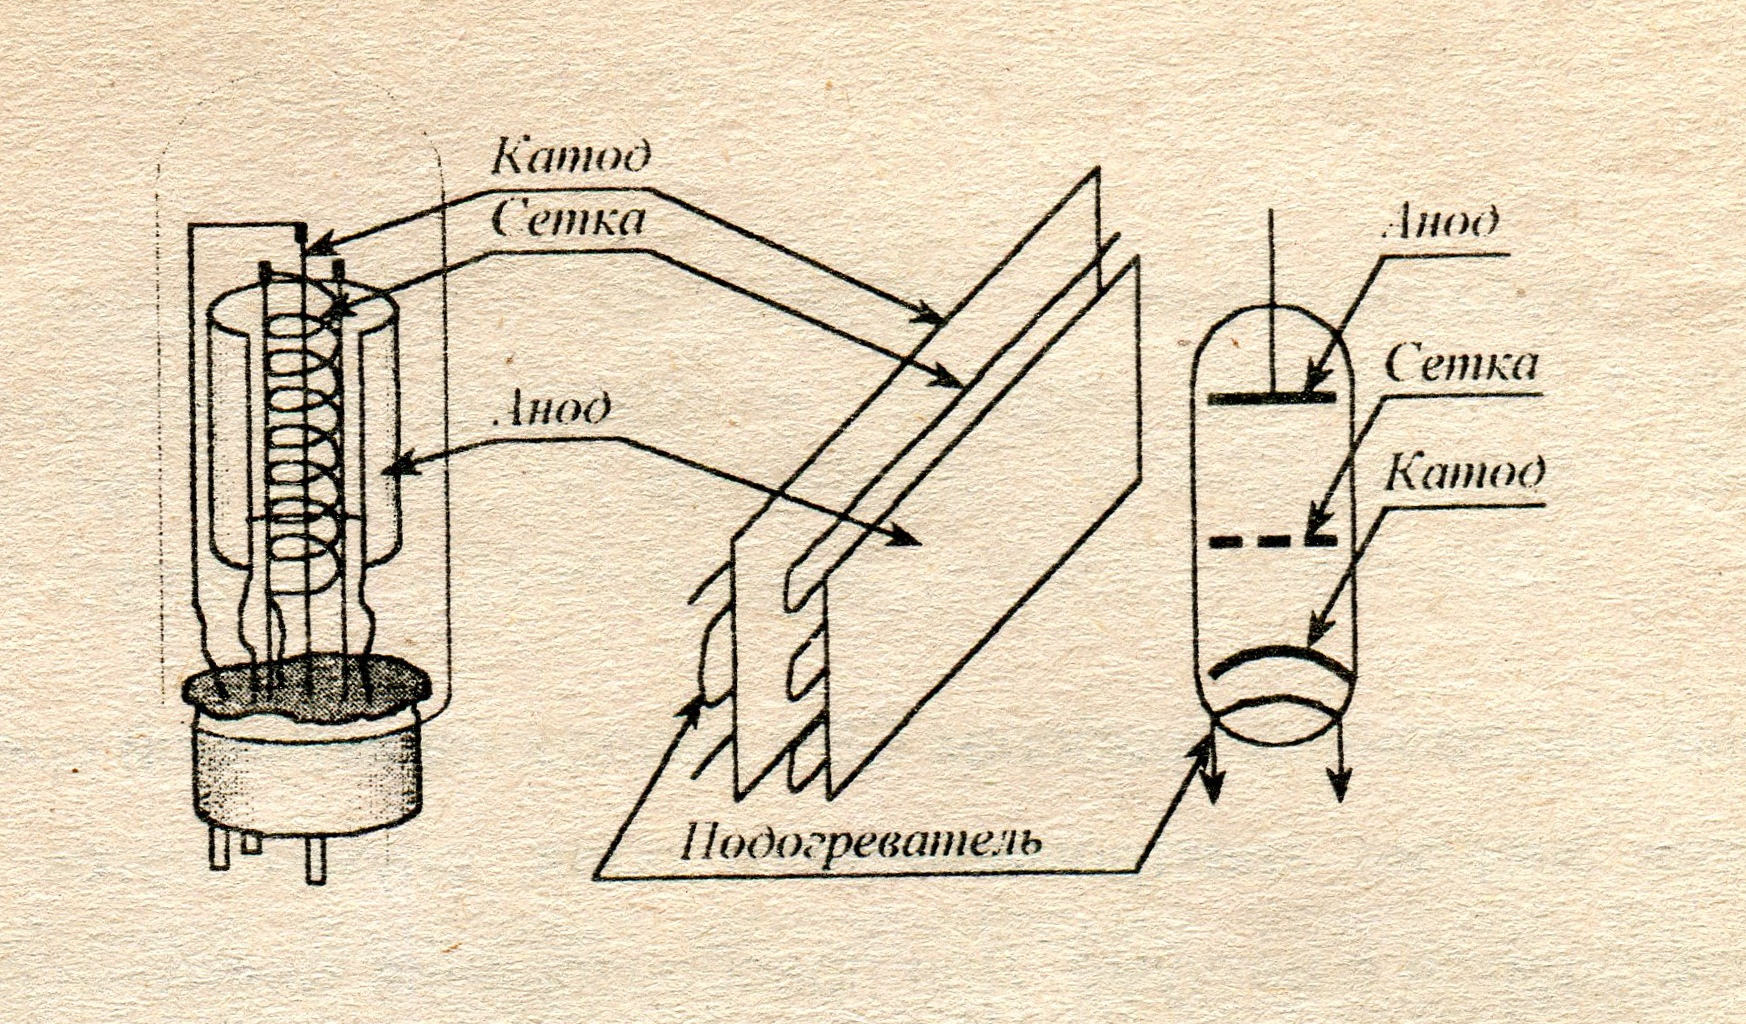
\includegraphics[width=0.8\linewidth]{fig/img3.jpg}
	\caption{Конструкция триода}
	\label{fig:1}
\end{figure}
Триод является усилителем тока, а при определенных условиях, - и напряжения. Основным рабочим режимом триода является, как и в диоде, режим ограничения тока пространственным зарядом. 

\subsection{Вольт-амперные характеристики триода}

Для описания свойств триода необходимо знать зависимости сеточного и анодного токов от подаваемых напряжений:
\begin{equation}
	J_a=J_a (U_c,U_a).
\end{equation}

\begin{equation}
	J_c=J_c (U_c,U_a).
\end{equation}

Наиболее важной для практических приложений является зависимость для анодного тока. Поскольку она является двумерной, для ее описания используют две одномерные зависимости:
\begin{equation}
	J_a=J_a (U_a), U_c=const
\end{equation}
и
\begin{equation}
	J_a=J_a (U_c), U_a=const
\end{equation}

Первая зависимость называется анодной характеристикой, вторая анодно-сеточной.

Можно показать, что для поля электродов плоского триода:
\begin{equation}
	E_{\text{эл}} = \frac{U_c+DU_a}{d_{kc}[1+D(1+d_{ca}/d_{kc})]},
\end{equation}
где 
\begin{equation}
	D \approx \frac{s}{2\pi d_{ca}}\ln{\frac{s}{2\pi \rho}}
\end{equation}

Коэффициент D определяет ту часть электрического поля вблизи катода, которая обусловлена присутствием анода и связана с "провисанием" потенциала $U_a$ через промежутки между витками сетки. Чем теснее расположены витки и чем толще проволока сетки, тем меньше D. Это позволяет назвать D проницаемостью сетки. Обычно $D \ll 1$, поэтому можно приближенно положить
\begin{equation}
	E = \frac{1}{d_{kc}}(U_c+DU_a)
\end{equation}

Тогда катодный ток в плоском триоде:
\begin{equation}
J_k=\frac49 \varepsilon_0 \sqrt{2 \eta} S_a \frac{(U_c+DU_a)^{3/2}}{d_{kc}^2}, 
\end{equation}
или в общем случае
\begin{equation}
J_k=P(U_c+DU_a)^{3/2}, 
\end{equation}
где  P-превеанс триода.

\subsection{Параметры триода}
Триод принято характеризовать тремя параметрами. Величина
\begin{equation}
	S= \pdv{J_a}{U_c} \eval _{U_a}, 
\end{equation}
является отношением бесконечно малых приращений анодного тока и напряжения на сетке и называется крутизной триода. 

Параметр 
\begin{equation}
	R= \pdv{U_a}{J_a} \eval _{U_c}, 
\end{equation}
называется внутренним сопротивлением. Геометрически этот параметр характеризует наклон анодных характеристик триода,
т.е. кривых, выражающих зависимость анодного тока от анодного напряжения при постоянном потенциале  
сетки.

Важным свйством триода, определяющим его способность усиливать напряжение является то, что малые 
изменения потенциала сетки эквивалентны в смысле воздействия на анодный ток большим изменениям 
потенциала анода, т.к. анод экранирован сеткой от катода и расположен от последнего дальше, 
чем сетка. Это свойство характеризуется коэффициентом усиления по напряжению:
\begin{equation}
	\mu= \pdv{U_a}{U_c} \eval _{J_a}, 
\end{equation}

Статические параметры не являются независимыми, а связаны соотношением:
\begin{equation}
	\mu= S \cdot R_i, 
\end{equation}
которое называется внутренним уравнением триода.

\section{Экспериментальная часть}
\subsection{Экспериментальная установка}
Схема установки:
\begin{figure}[h!]
	\centering
	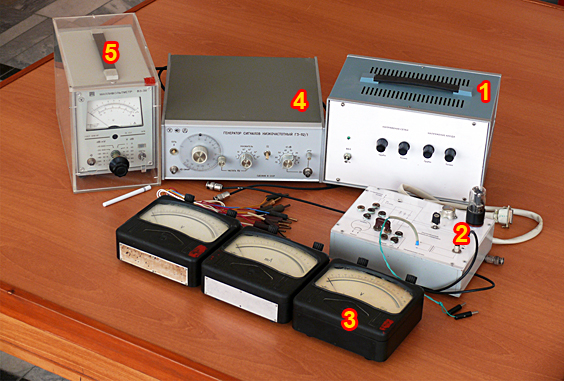
\includegraphics[width=0.5\linewidth]{fig/img4.jpg}
	\caption{Схема экспериментальной установки}
	\label{fig:10}
\end{figure}

Блок режимов (1) обеспечивает требуемые напряжения на электродах исследуемой электронной 
лампы-триода. Исследуемый триод размещается на верхней панели измерительного блока (2), 
там же расположены элементы коммутации, позволяющие изменять схему включения триода. Для 
контроля режима лампы по постоянному току используются стрелочные лабораторные вольтметры 
и миллиамперметр ЛМ-1 (3). Звуковой генератор Г3-112 (4) обеспечивает подачу переменного 
напряжения для реализации метода переменной составляющей. Для измерения значений переменного 
напряжения используется аналоговый милливольтметр переменного тока В3-38 (5).

\subsection{Задание 1}
\begin{figure}[h!]
 	\centering
	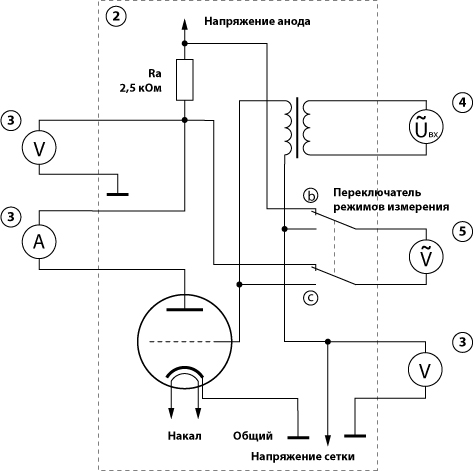
\includegraphics[width=0.5\linewidth]{fig/img5.jpg}
 	\caption{К заданию 1}
 	\label{fig:11}
\end{figure}

Проведите измерения следующих зависимостей:

а) Ia = f(Uс) при Uа = 220 В; 

б) Ia = f(Uс) при Uа = 150 В;

в) S = f(Uс) при Uа = 220 В; 

г) S = f(Uа) при Uс = -8 В.

\subsection{Задание 2}
\begin{figure}[h!]
 	\centering
	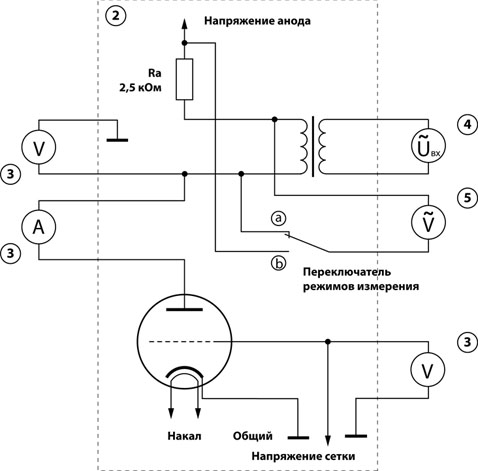
\includegraphics[width=0.5\linewidth]{fig/img6.jpg}
 	\caption{К заданию 2}
 	\label{fig:11}
\end{figure}

Проведите измерения следующих зависимостей:

а) Ia = f(Uа) при Uс = - 8 В;

б) Ia = f(Uа) при Uс = - 6 В;

в) Ri = f(Uа) при Uс = - 8 В;

г) Ri = f(Uc) при Ua = 220 В.

\subsection{Задание 3}
По результатам измерений постройте графики зависимости от напряжения на сетке и на 
аноде ламы:

а) анодного тока
\begin{figure}[h!]
	\centering
	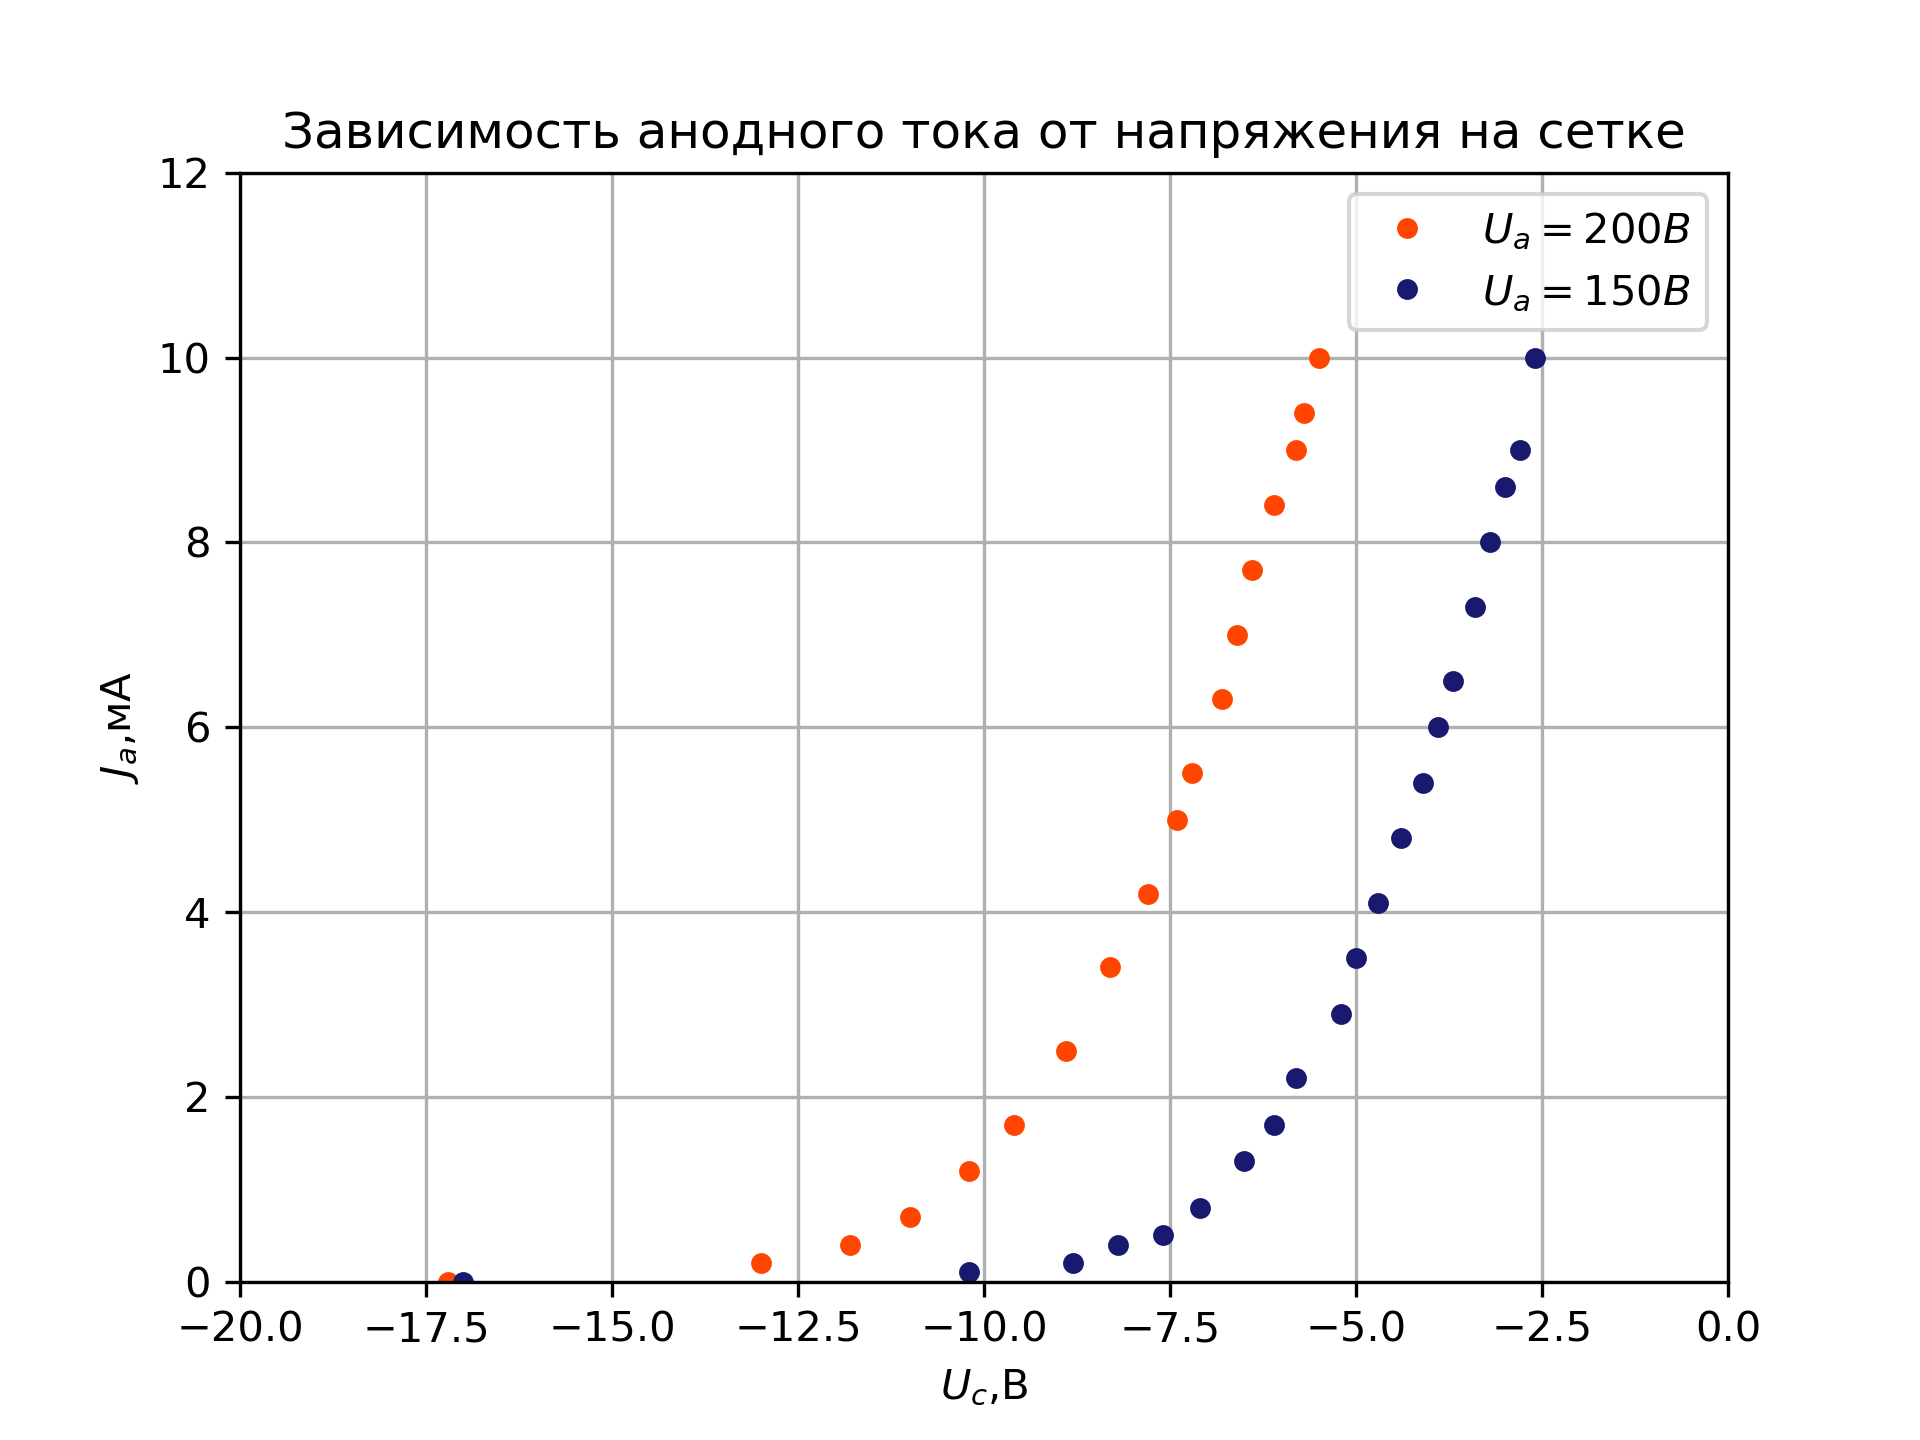
\includegraphics[width=0.7\linewidth]{scripts/z01.png}
	\caption{}
	\label{fig:10}
\end{figure}

\begin{figure}[h!]
	\centering
	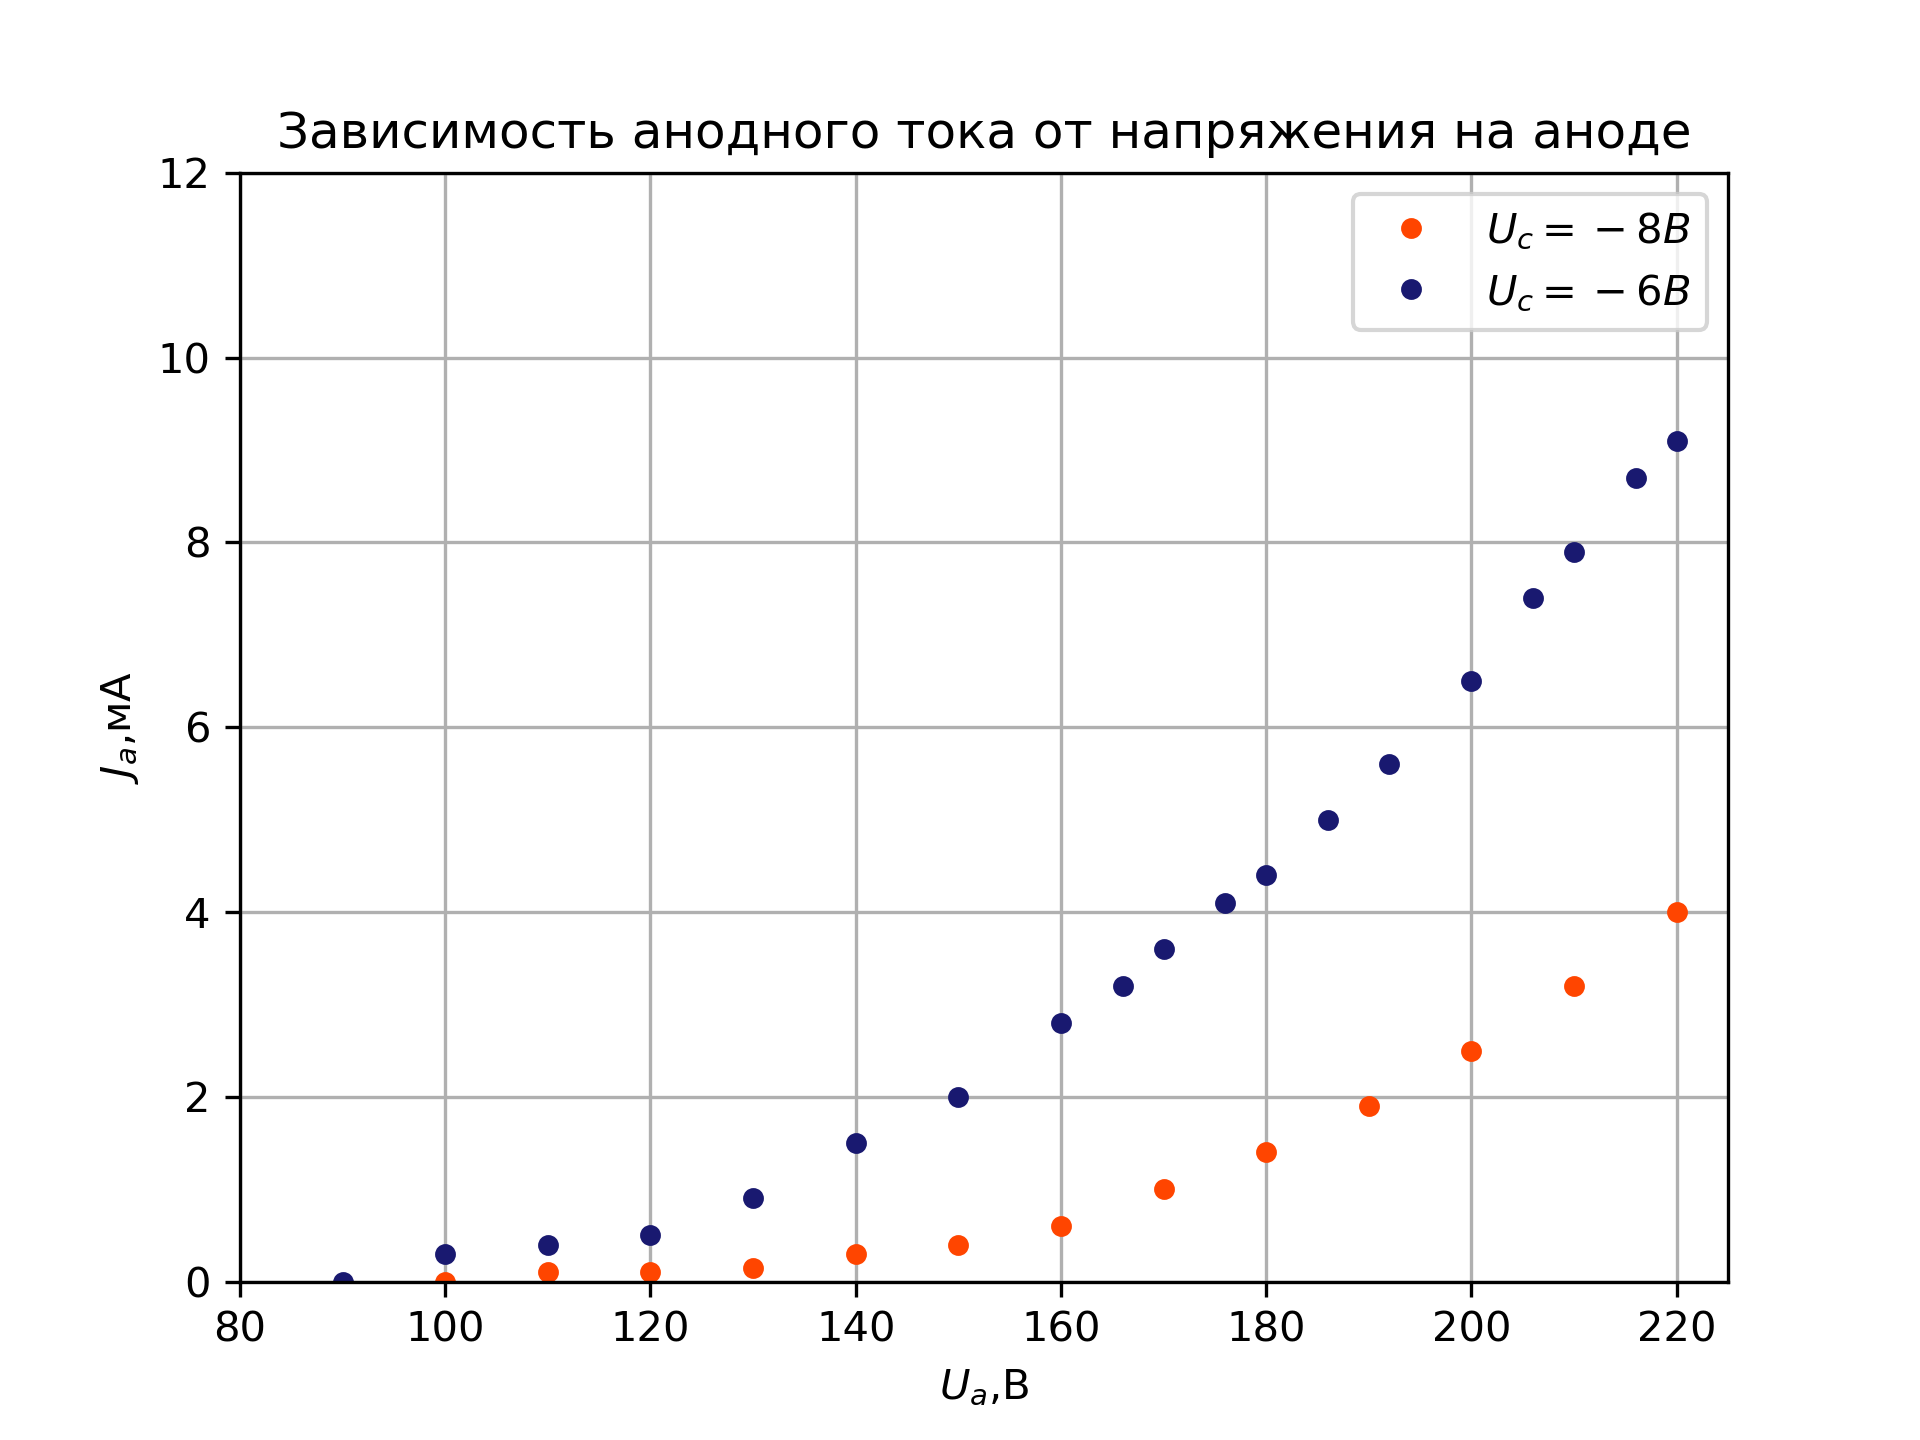
\includegraphics[width=0.7\linewidth]{scripts/z02.png}
	\caption{}
	\label{fig:10}
\end{figure}

б) крутизны
\begin{figure}[h!]
	\centering
	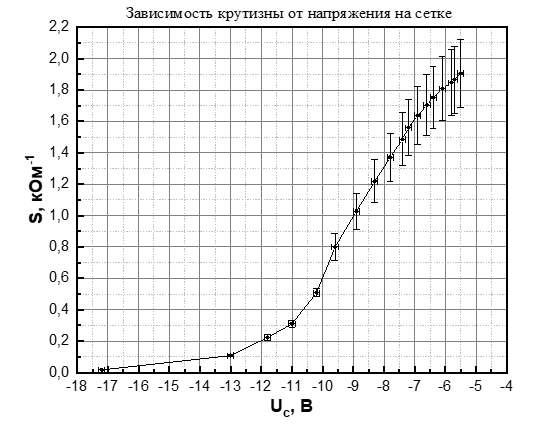
\includegraphics[width=0.7\linewidth]{fig/img11.png}
	\caption{}
	\label{fig:10}
\end{figure}

\begin{figure}[H]
	\centering
	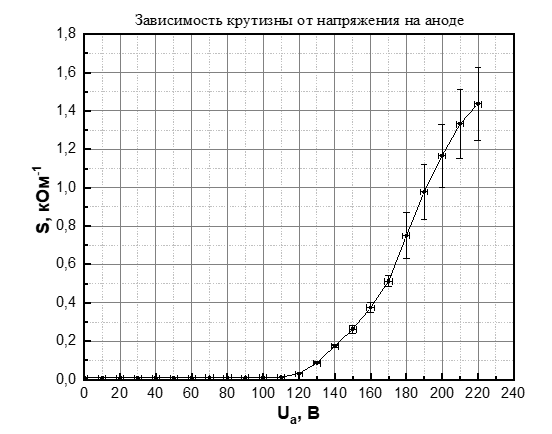
\includegraphics[width=0.7\linewidth]{fig/img12.png}
	\caption{}
	\label{fig:10}
\end{figure}

в) внутреннего сопротивления
\begin{figure}[h!]
	\centering
	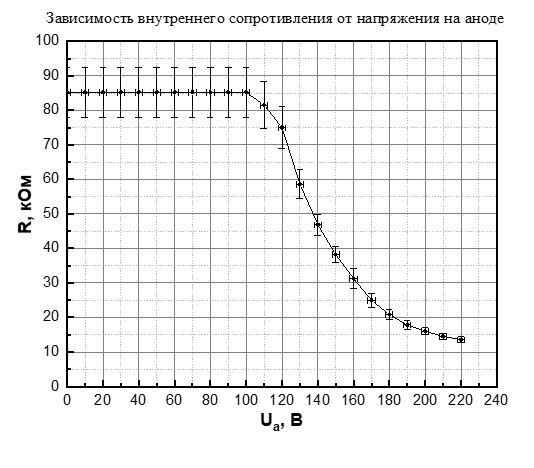
\includegraphics[width=0.7\linewidth]{fig/img21.png}
	\caption{}
	\label{fig:10}
\end{figure}

\begin{figure}[H]
	\centering
	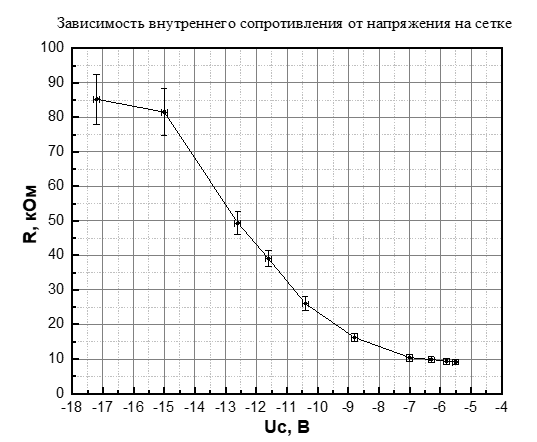
\includegraphics[width=0.7\linewidth]{fig/img22.png}
	\caption{}
	\label{fig:10}
\end{figure}

г) статического коэффициента усиления по напряжению
\begin{figure}[h!]
	\centering
	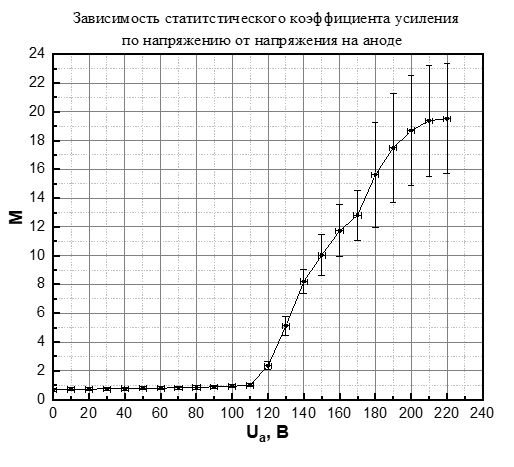
\includegraphics[width=0.65\linewidth]{fig/img31.png}
	\caption{}
	\label{fig:10}
\end{figure}

\begin{figure}[H]
	\centering
	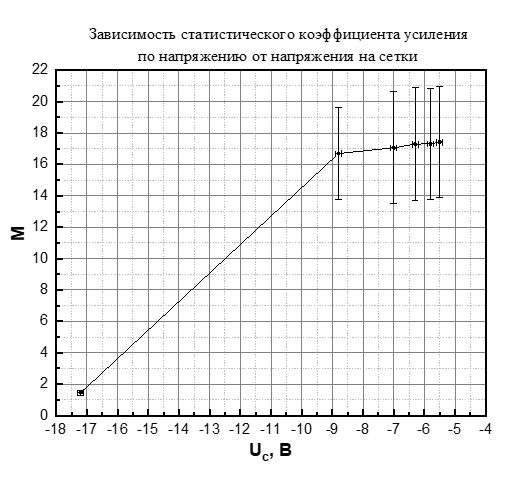
\includegraphics[width=0.7\linewidth]{fig/img32.png}
	\caption{}
	\label{fig:10}
\end{figure}


Погрешность анодного напряжения $\Delta U_a = 2 B$.

Погрешность анодного тока $\Delta J_a = 0.1 mA$.

Погрешность сеточного напряжения $\Delta U_c = 0.1 B$.

Формулы для рассчета погрешности крутизны:
\begin{gather*}
	S=\frac{U_{out}}{U_{in}} \frac{1}{R_a}, \\
	\Delta S=  \frac{1}{R_a U_{in}}(\Delta U_{out}+\frac{U_{out}}{U_{in}}\Delta U_{in}). 
\end{gather*}

и внутреннего сопротивления:
\begin{gather*}
	R=\frac{U_{in}}{U_{out}} R_a, \\
	\Delta R=  \frac{R_a}{U_{out}}(\Delta U_{in}+\frac{U_{in}}{U_{out}}\Delta U_{out}). 
\end{gather*}

\end{document}
